% ======================================================================
%  Shared style for the master CV (cv-en.tex and cv-de.tex)
%
%  Layout follows the previous CV (Jake Gutierrez's resume template, MIT
%  licence), adapted to A4 and tuned for applicant tracking systems (ATS):
%    - one column, standard section names, real text only
%    - no icon fonts (they extract as garbage characters)
%    - every glyph mapped to Unicode, f-ligatures switched off
%    - PDF title, author and keywords set
%
%  Before % ======================================================================
%  Shared style for the master CV (cv-en.tex and cv-de.tex)
%
%  Layout follows the previous CV (Jake Gutierrez's resume template, MIT
%  licence), adapted to A4 and tuned for applicant tracking systems (ATS):
%    - one column, standard section names, real text only
%    - no icon fonts (they extract as garbage characters)
%    - every glyph mapped to Unicode, f-ligatures switched off
%    - PDF title, author and keywords set
%
%  Before % ======================================================================
%  Shared style for the master CV (cv-en.tex and cv-de.tex)
%
%  Layout follows the previous CV (Jake Gutierrez's resume template, MIT
%  licence), adapted to A4 and tuned for applicant tracking systems (ATS):
%    - one column, standard section names, real text only
%    - no icon fonts (they extract as garbage characters)
%    - every glyph mapped to Unicode, f-ligatures switched off
%    - PDF title, author and keywords set
%
%  Before % ======================================================================
%  Shared style for the master CV (cv-en.tex and cv-de.tex)
%
%  Layout follows the previous CV (Jake Gutierrez's resume template, MIT
%  licence), adapted to A4 and tuned for applicant tracking systems (ATS):
%    - one column, standard section names, real text only
%    - no icon fonts (they extract as garbage characters)
%    - every glyph mapped to Unicode, f-ligatures switched off
%    - PDF title, author and keywords set
%
%  Before \input{cv-style} the main file must define:
%    \cvlang      babel language (english or ngerman)
%    \cvpdflang   PDF language tag (en-GB or de-DE)
%    \cvdoctitle  document title for the PDF metadata
%    \cvpageword  the word for "page" in the footer
% ======================================================================

\usepackage[T1]{fontenc}
\usepackage[utf8]{inputenc}
\usepackage[\cvlang]{babel}
\usepackage{lmodern}
\usepackage[a4paper,left=1.45cm,right=1.45cm,top=1.1cm,bottom=1.45cm,footskip=0.7cm]{geometry}
\usepackage{titlesec}
\usepackage{enumitem}
\usepackage{graphicx}
\usepackage{xcolor}
\usepackage{fancyhdr}
\usepackage{lastpage}
\usepackage{microtype}
\usepackage[hidelinks]{hyperref}

% ---------- ATS: machine-readable text ----------
\input{glyphtounicode}
\pdfgentounicode=1
\DisableLigatures[f]{encoding = *, family = *}

% ---------- Personal data (edit once, used by both languages) ----------
\newcommand{\cvname}{Somantha Manuranga}
\newcommand{\cvphone}{+49 174 7656939}
\newcommand{\cvemail}{somanthamanuranga@gmail.com}
\newcommand{\cvlinkedin}{linkedin.com/in/somantha-manuranga-b73432192}
\newcommand{\cvgithub}{github.com/SomanthaManuranga}
\newcommand{\cvportfolio}{somanthamanuranga.github.io/portfolio}

% Set to \photofalse for a version without a photo (some online
% application forms and international employers prefer that).
\newif\ifphoto
\phototrue

\hypersetup{
  pdftitle={\cvname\ - \cvdoctitle},
  pdfauthor={\cvname},
  pdfsubject={\cvdoctitle},
  pdfkeywords={AI Engineer, Machine Learning, Deep Learning, Computer Vision, NLP, LLM, PyTorch, Python, Industrial AI, Werkstudent},
  pdflang={\cvpdflang},
}

% ---------- Page ----------
\pagestyle{fancy}
\fancyhf{}
\renewcommand{\headrulewidth}{0pt}
\renewcommand{\footrulewidth}{0pt}
\fancyfoot[C]{\footnotesize\color{black!55}\cvname\ \textperiodcentered\ \cvpageword\ \thepage\ / \pageref*{LastPage}}
\setlength{\parindent}{0pt}
\setlength{\tabcolsep}{0pt}
\raggedbottom
\raggedright
\urlstyle{same}

% ---------- Section headings: small caps with a rule ----------
\titleformat{\section}{\vspace{-5pt}\scshape\raggedright\large}{}{0em}{}[\color{black}\titlerule\vspace{-5pt}]
\titlespacing*{\section}{0pt}{9pt}{7pt}

% ---------- Building blocks ----------
% \cvheader{line 1}{line 2}{line 3}{line 4}
% Each contact detail sits in an \mbox so that it is never hyphenated or
% split across lines (a broken email address or URL confuses ATS parsers).
\newcommand{\cvheader}[4]{%
  \begin{minipage}[c]{0.78\textwidth}
    {\Huge\bfseries \cvname}\\[6pt]
    {\small #1}\\[1.5pt]
    {\small #2}\\[1.5pt]
    {\small #3}\\[1.5pt]
    {\small #4}
  \end{minipage}%
  \hfill
  \ifphoto
  \begin{minipage}[c]{0.19\textwidth}
    \raggedleft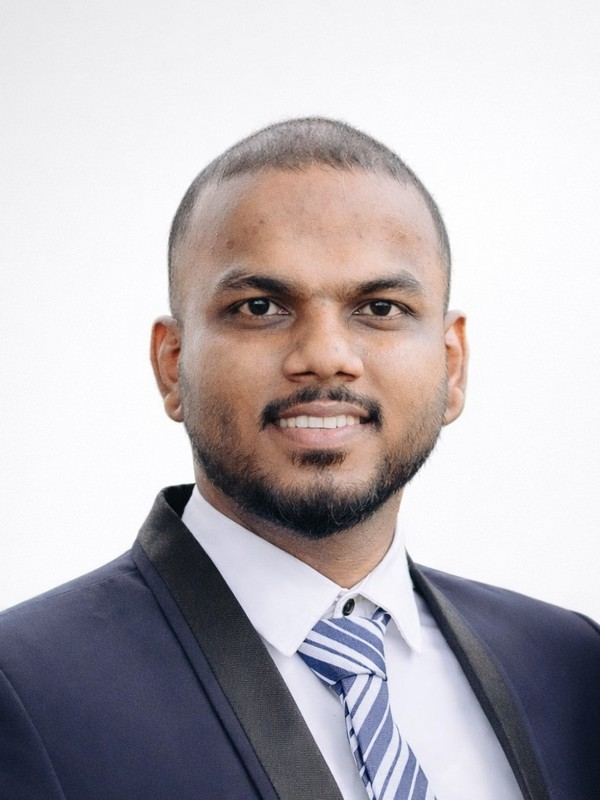
\includegraphics[width=2.75cm]{photo.jpg}
  \end{minipage}%
  \fi
  \par\vspace{3pt}
}
\newcommand{\cvsep}{\hspace{5pt}\textbullet\hspace{5pt}}

% Entry lists
\newcommand{\cvliststart}{\begin{itemize}[leftmargin=0.25cm, label={}, itemsep=3pt, topsep=0pt, parsep=0pt]}
\newcommand{\cvlistend}{\end{itemize}}

% \cventry{organisation}{location}{role or degree}{dates}
\newcommand{\cventry}[4]{%
  \item
  \begin{tabular*}{\linewidth}[t]{l@{\extracolsep{\fill}}r}
    \textbf{#1} & {\small #2} \\
    \textit{\small #3} & \textit{\small #4} \\
  \end{tabular*}\nopagebreak\vspace{-2pt}
}

% \cvproject{name}{technologies}{year}
\newcommand{\cvproject}[3]{%
  \item
  \begin{tabular*}{\linewidth}[t]{l@{\extracolsep{\fill}}r}
    {\small\textbf{#1} $|$ \textit{#2}} & \textit{\small #3} \\
  \end{tabular*}\nopagebreak\vspace{-2pt}
}

% \cvgroup{label}: sub-heading inside the project list
\newcommand{\cvgroup}[1]{\item[] \vspace{1pt}{\small\bfseries\itshape #1}\vspace{-1pt}}

% Bullet points under an entry
\newcommand{\cvpointsstart}{\begin{itemize}[leftmargin=0.45cm, label=\textbullet, itemsep=0.5pt, topsep=1pt, parsep=0pt]\small}
\newcommand{\cvpointsend}{\end{itemize}}

% \cvline{label}{text}: one line in the skills-style sections
\newcommand{\cvline}[2]{\item {\small \textbf{#1:} #2}}
 the main file must define:
%    \cvlang      babel language (english or ngerman)
%    \cvpdflang   PDF language tag (en-GB or de-DE)
%    \cvdoctitle  document title for the PDF metadata
%    \cvpageword  the word for "page" in the footer
% ======================================================================

\usepackage[T1]{fontenc}
\usepackage[utf8]{inputenc}
\usepackage[\cvlang]{babel}
\usepackage{lmodern}
\usepackage[a4paper,left=1.45cm,right=1.45cm,top=1.1cm,bottom=1.45cm,footskip=0.7cm]{geometry}
\usepackage{titlesec}
\usepackage{enumitem}
\usepackage{graphicx}
\usepackage{xcolor}
\usepackage{fancyhdr}
\usepackage{lastpage}
\usepackage{microtype}
\usepackage[hidelinks]{hyperref}

% ---------- ATS: machine-readable text ----------
\input{glyphtounicode}
\pdfgentounicode=1
\DisableLigatures[f]{encoding = *, family = *}

% ---------- Personal data (edit once, used by both languages) ----------
\newcommand{\cvname}{Somantha Manuranga}
\newcommand{\cvphone}{+49 174 7656939}
\newcommand{\cvemail}{somanthamanuranga@gmail.com}
\newcommand{\cvlinkedin}{linkedin.com/in/somantha-manuranga-b73432192}
\newcommand{\cvgithub}{github.com/SomanthaManuranga}
\newcommand{\cvportfolio}{somanthamanuranga.github.io/portfolio}

% Set to \photofalse for a version without a photo (some online
% application forms and international employers prefer that).
\newif\ifphoto
\phototrue

\hypersetup{
  pdftitle={\cvname\ - \cvdoctitle},
  pdfauthor={\cvname},
  pdfsubject={\cvdoctitle},
  pdfkeywords={AI Engineer, Machine Learning, Deep Learning, Computer Vision, NLP, LLM, PyTorch, Python, Industrial AI, Werkstudent},
  pdflang={\cvpdflang},
}

% ---------- Page ----------
\pagestyle{fancy}
\fancyhf{}
\renewcommand{\headrulewidth}{0pt}
\renewcommand{\footrulewidth}{0pt}
\fancyfoot[C]{\footnotesize\color{black!55}\cvname\ \textperiodcentered\ \cvpageword\ \thepage\ / \pageref*{LastPage}}
\setlength{\parindent}{0pt}
\setlength{\tabcolsep}{0pt}
\raggedbottom
\raggedright
\urlstyle{same}

% ---------- Section headings: small caps with a rule ----------
\titleformat{\section}{\vspace{-5pt}\scshape\raggedright\large}{}{0em}{}[\color{black}\titlerule\vspace{-5pt}]
\titlespacing*{\section}{0pt}{9pt}{7pt}

% ---------- Building blocks ----------
% \cvheader{line 1}{line 2}{line 3}{line 4}
% Each contact detail sits in an \mbox so that it is never hyphenated or
% split across lines (a broken email address or URL confuses ATS parsers).
\newcommand{\cvheader}[4]{%
  \begin{minipage}[c]{0.78\textwidth}
    {\Huge\bfseries \cvname}\\[6pt]
    {\small #1}\\[1.5pt]
    {\small #2}\\[1.5pt]
    {\small #3}\\[1.5pt]
    {\small #4}
  \end{minipage}%
  \hfill
  \ifphoto
  \begin{minipage}[c]{0.19\textwidth}
    \raggedleft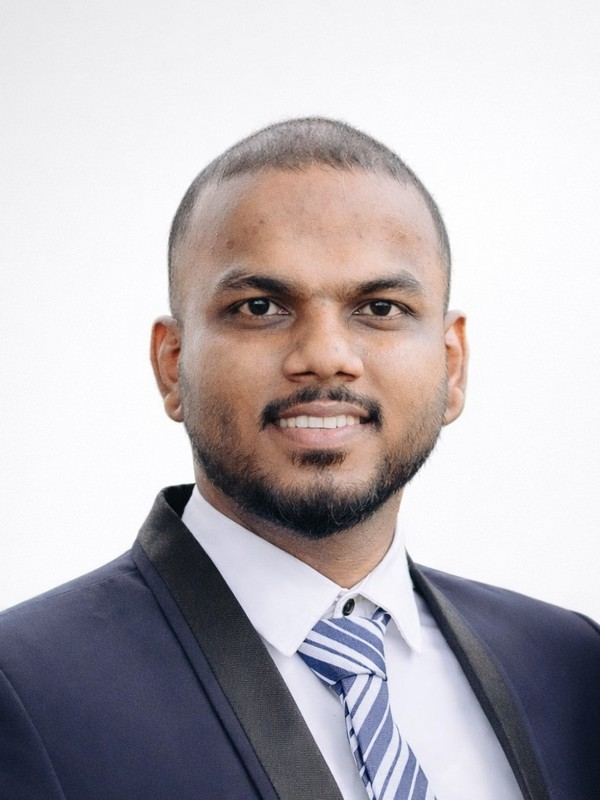
\includegraphics[width=2.75cm]{photo.jpg}
  \end{minipage}%
  \fi
  \par\vspace{3pt}
}
\newcommand{\cvsep}{\hspace{5pt}\textbullet\hspace{5pt}}

% Entry lists
\newcommand{\cvliststart}{\begin{itemize}[leftmargin=0.25cm, label={}, itemsep=3pt, topsep=0pt, parsep=0pt]}
\newcommand{\cvlistend}{\end{itemize}}

% \cventry{organisation}{location}{role or degree}{dates}
\newcommand{\cventry}[4]{%
  \item
  \begin{tabular*}{\linewidth}[t]{l@{\extracolsep{\fill}}r}
    \textbf{#1} & {\small #2} \\
    \textit{\small #3} & \textit{\small #4} \\
  \end{tabular*}\nopagebreak\vspace{-2pt}
}

% \cvproject{name}{technologies}{year}
\newcommand{\cvproject}[3]{%
  \item
  \begin{tabular*}{\linewidth}[t]{l@{\extracolsep{\fill}}r}
    {\small\textbf{#1} $|$ \textit{#2}} & \textit{\small #3} \\
  \end{tabular*}\nopagebreak\vspace{-2pt}
}

% \cvgroup{label}: sub-heading inside the project list
\newcommand{\cvgroup}[1]{\item[] \vspace{1pt}{\small\bfseries\itshape #1}\vspace{-1pt}}

% Bullet points under an entry
\newcommand{\cvpointsstart}{\begin{itemize}[leftmargin=0.45cm, label=\textbullet, itemsep=0.5pt, topsep=1pt, parsep=0pt]\small}
\newcommand{\cvpointsend}{\end{itemize}}

% \cvline{label}{text}: one line in the skills-style sections
\newcommand{\cvline}[2]{\item {\small \textbf{#1:} #2}}
 the main file must define:
%    \cvlang      babel language (english or ngerman)
%    \cvpdflang   PDF language tag (en-GB or de-DE)
%    \cvdoctitle  document title for the PDF metadata
%    \cvpageword  the word for "page" in the footer
% ======================================================================

\usepackage[T1]{fontenc}
\usepackage[utf8]{inputenc}
\usepackage[\cvlang]{babel}
\usepackage{lmodern}
\usepackage[a4paper,left=1.45cm,right=1.45cm,top=1.1cm,bottom=1.45cm,footskip=0.7cm]{geometry}
\usepackage{titlesec}
\usepackage{enumitem}
\usepackage{graphicx}
\usepackage{xcolor}
\usepackage{fancyhdr}
\usepackage{lastpage}
\usepackage{microtype}
\usepackage[hidelinks]{hyperref}

% ---------- ATS: machine-readable text ----------
\input{glyphtounicode}
\pdfgentounicode=1
\DisableLigatures[f]{encoding = *, family = *}

% ---------- Personal data (edit once, used by both languages) ----------
\newcommand{\cvname}{Somantha Manuranga}
\newcommand{\cvphone}{+49 174 7656939}
\newcommand{\cvemail}{somanthamanuranga@gmail.com}
\newcommand{\cvlinkedin}{linkedin.com/in/somantha-manuranga-b73432192}
\newcommand{\cvgithub}{github.com/SomanthaManuranga}
\newcommand{\cvportfolio}{somanthamanuranga.github.io/portfolio}

% Set to \photofalse for a version without a photo (some online
% application forms and international employers prefer that).
\newif\ifphoto
\phototrue

\hypersetup{
  pdftitle={\cvname\ - \cvdoctitle},
  pdfauthor={\cvname},
  pdfsubject={\cvdoctitle},
  pdfkeywords={AI Engineer, Machine Learning, Deep Learning, Computer Vision, NLP, LLM, PyTorch, Python, Industrial AI, Werkstudent},
  pdflang={\cvpdflang},
}

% ---------- Page ----------
\pagestyle{fancy}
\fancyhf{}
\renewcommand{\headrulewidth}{0pt}
\renewcommand{\footrulewidth}{0pt}
\fancyfoot[C]{\footnotesize\color{black!55}\cvname\ \textperiodcentered\ \cvpageword\ \thepage\ / \pageref*{LastPage}}
\setlength{\parindent}{0pt}
\setlength{\tabcolsep}{0pt}
\raggedbottom
\raggedright
\urlstyle{same}

% ---------- Section headings: small caps with a rule ----------
\titleformat{\section}{\vspace{-5pt}\scshape\raggedright\large}{}{0em}{}[\color{black}\titlerule\vspace{-5pt}]
\titlespacing*{\section}{0pt}{9pt}{7pt}

% ---------- Building blocks ----------
% \cvheader{line 1}{line 2}{line 3}{line 4}
% Each contact detail sits in an \mbox so that it is never hyphenated or
% split across lines (a broken email address or URL confuses ATS parsers).
\newcommand{\cvheader}[4]{%
  \begin{minipage}[c]{0.78\textwidth}
    {\Huge\bfseries \cvname}\\[6pt]
    {\small #1}\\[1.5pt]
    {\small #2}\\[1.5pt]
    {\small #3}\\[1.5pt]
    {\small #4}
  \end{minipage}%
  \hfill
  \ifphoto
  \begin{minipage}[c]{0.19\textwidth}
    \raggedleft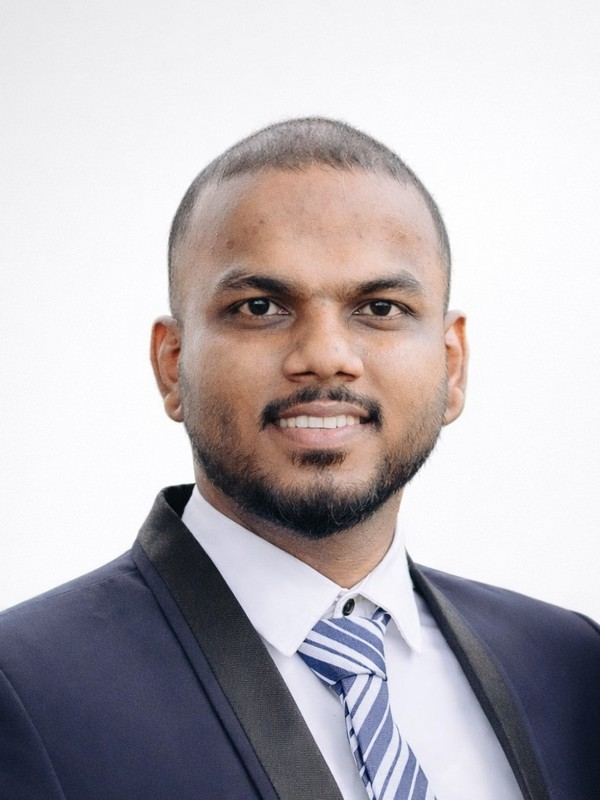
\includegraphics[width=2.75cm]{photo.jpg}
  \end{minipage}%
  \fi
  \par\vspace{3pt}
}
\newcommand{\cvsep}{\hspace{5pt}\textbullet\hspace{5pt}}

% Entry lists
\newcommand{\cvliststart}{\begin{itemize}[leftmargin=0.25cm, label={}, itemsep=3pt, topsep=0pt, parsep=0pt]}
\newcommand{\cvlistend}{\end{itemize}}

% \cventry{organisation}{location}{role or degree}{dates}
\newcommand{\cventry}[4]{%
  \item
  \begin{tabular*}{\linewidth}[t]{l@{\extracolsep{\fill}}r}
    \textbf{#1} & {\small #2} \\
    \textit{\small #3} & \textit{\small #4} \\
  \end{tabular*}\nopagebreak\vspace{-2pt}
}

% \cvproject{name}{technologies}{year}
\newcommand{\cvproject}[3]{%
  \item
  \begin{tabular*}{\linewidth}[t]{l@{\extracolsep{\fill}}r}
    {\small\textbf{#1} $|$ \textit{#2}} & \textit{\small #3} \\
  \end{tabular*}\nopagebreak\vspace{-2pt}
}

% \cvgroup{label}: sub-heading inside the project list
\newcommand{\cvgroup}[1]{\item[] \vspace{1pt}{\small\bfseries\itshape #1}\vspace{-1pt}}

% Bullet points under an entry
\newcommand{\cvpointsstart}{\begin{itemize}[leftmargin=0.45cm, label=\textbullet, itemsep=0.5pt, topsep=1pt, parsep=0pt]\small}
\newcommand{\cvpointsend}{\end{itemize}}

% \cvline{label}{text}: one line in the skills-style sections
\newcommand{\cvline}[2]{\item {\small \textbf{#1:} #2}}
 the main file must define:
%    \cvlang      babel language (english or ngerman)
%    \cvpdflang   PDF language tag (en-GB or de-DE)
%    \cvdoctitle  document title for the PDF metadata
%    \cvpageword  the word for "page" in the footer
% ======================================================================

\usepackage[T1]{fontenc}
\usepackage[utf8]{inputenc}
\usepackage[\cvlang]{babel}
\usepackage{lmodern}
\usepackage[a4paper,left=1.45cm,right=1.45cm,top=1.1cm,bottom=1.45cm,footskip=0.7cm]{geometry}
\usepackage{titlesec}
\usepackage{enumitem}
\usepackage{graphicx}
\usepackage{xcolor}
\usepackage{fancyhdr}
\usepackage{lastpage}
\usepackage{microtype}
\usepackage[hidelinks]{hyperref}

% ---------- ATS: machine-readable text ----------
\input{glyphtounicode}
\pdfgentounicode=1
\DisableLigatures[f]{encoding = *, family = *}

% ---------- Personal data (edit once, used by both languages) ----------
\newcommand{\cvname}{Somantha Manuranga}
\newcommand{\cvphone}{+49 174 7656939}
\newcommand{\cvemail}{somanthamanuranga@gmail.com}
\newcommand{\cvlinkedin}{linkedin.com/in/somantha-manuranga-b73432192}
\newcommand{\cvgithub}{github.com/SomanthaManuranga}
\newcommand{\cvportfolio}{somanthamanuranga.github.io/portfolio}

% Set to \photofalse for a version without a photo (some online
% application forms and international employers prefer that).
\newif\ifphoto
\phototrue

\hypersetup{
  pdftitle={\cvname\ - \cvdoctitle},
  pdfauthor={\cvname},
  pdfsubject={\cvdoctitle},
  pdfkeywords={AI Engineer, Machine Learning, Deep Learning, Computer Vision, NLP, LLM, PyTorch, Python, Industrial AI, Werkstudent},
  pdflang={\cvpdflang},
}

% ---------- Page ----------
\pagestyle{fancy}
\fancyhf{}
\renewcommand{\headrulewidth}{0pt}
\renewcommand{\footrulewidth}{0pt}
\fancyfoot[C]{\footnotesize\color{black!55}\cvname\ \textperiodcentered\ \cvpageword\ \thepage\ / \pageref*{LastPage}}
\setlength{\parindent}{0pt}
\setlength{\tabcolsep}{0pt}
\raggedbottom
\raggedright
\urlstyle{same}

% ---------- Section headings: small caps with a rule ----------
\titleformat{\section}{\vspace{-5pt}\scshape\raggedright\large}{}{0em}{}[\color{black}\titlerule\vspace{-5pt}]
\titlespacing*{\section}{0pt}{9pt}{7pt}

% ---------- Building blocks ----------
% \cvheader{line 1}{line 2}{line 3}{line 4}
% Each contact detail sits in an \mbox so that it is never hyphenated or
% split across lines (a broken email address or URL confuses ATS parsers).
\newcommand{\cvheader}[4]{%
  \begin{minipage}[c]{0.78\textwidth}
    {\Huge\bfseries \cvname}\\[6pt]
    {\small #1}\\[1.5pt]
    {\small #2}\\[1.5pt]
    {\small #3}\\[1.5pt]
    {\small #4}
  \end{minipage}%
  \hfill
  \ifphoto
  \begin{minipage}[c]{0.19\textwidth}
    \raggedleft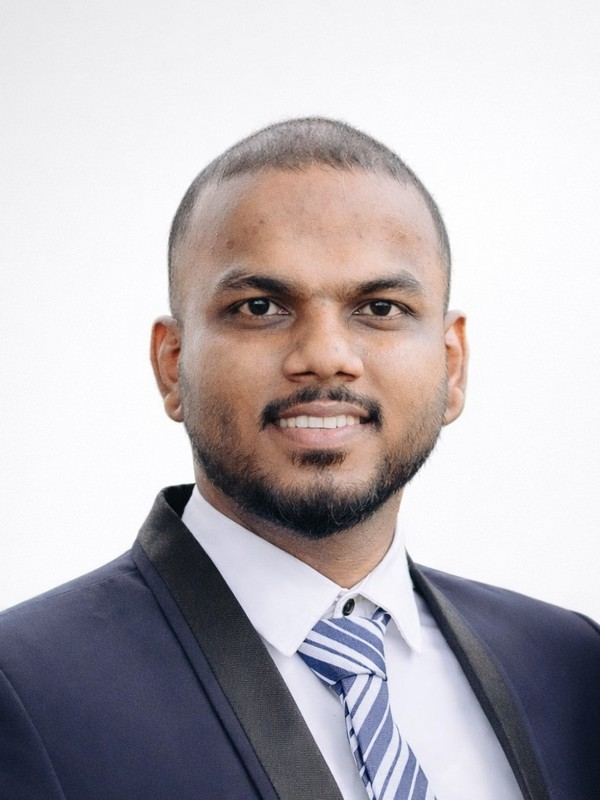
\includegraphics[width=2.75cm]{photo.jpg}
  \end{minipage}%
  \fi
  \par\vspace{3pt}
}
\newcommand{\cvsep}{\hspace{5pt}\textbullet\hspace{5pt}}

% Entry lists
\newcommand{\cvliststart}{\begin{itemize}[leftmargin=0.25cm, label={}, itemsep=3pt, topsep=0pt, parsep=0pt]}
\newcommand{\cvlistend}{\end{itemize}}

% \cventry{organisation}{location}{role or degree}{dates}
\newcommand{\cventry}[4]{%
  \item
  \begin{tabular*}{\linewidth}[t]{l@{\extracolsep{\fill}}r}
    \textbf{#1} & {\small #2} \\
    \textit{\small #3} & \textit{\small #4} \\
  \end{tabular*}\nopagebreak\vspace{-2pt}
}

% \cvproject{name}{technologies}{year}
\newcommand{\cvproject}[3]{%
  \item
  \begin{tabular*}{\linewidth}[t]{l@{\extracolsep{\fill}}r}
    {\small\textbf{#1} $|$ \textit{#2}} & \textit{\small #3} \\
  \end{tabular*}\nopagebreak\vspace{-2pt}
}

% \cvgroup{label}: sub-heading inside the project list
\newcommand{\cvgroup}[1]{\item[] \vspace{1pt}{\small\bfseries\itshape #1}\vspace{-1pt}}

% Bullet points under an entry
\newcommand{\cvpointsstart}{\begin{itemize}[leftmargin=0.45cm, label=\textbullet, itemsep=0.5pt, topsep=1pt, parsep=0pt]\small}
\newcommand{\cvpointsend}{\end{itemize}}

% \cvline{label}{text}: one line in the skills-style sections
\newcommand{\cvline}[2]{\item {\small \textbf{#1:} #2}}
